% Created 2021-02-24 Wed 14:07
% Intended LaTeX compiler: pdflatex
\documentclass[11pt]{article}
\usepackage[utf8]{inputenc}
\usepackage[T1]{fontenc}
\usepackage{graphicx}
\usepackage{grffile}
\usepackage{longtable}
\usepackage{wrapfig}
\usepackage{rotating}
\usepackage[normalem]{ulem}
\usepackage{amsmath}
\usepackage{textcomp}
\usepackage{amssymb}
\usepackage{capt-of}
\usepackage{hyperref}
\usepackage{minted}
\usepackage[margin=1in]{geometry}
\usepackage{subcaption}
\date{}
\title{Status update}
\hypersetup{
 pdfauthor={Alexey Bochkarev},
 pdftitle={Status update},
 pdfkeywords={},
 pdfsubject={},
 pdfcreator={Emacs 28.0.50 (Org mode 9.4.3)}, 
 pdflang={English}}
\begin{document}

\maketitle

\section{Status}
\label{sec:orgb174723}
\begin{itemize}
\item I have implemented some of the key machinery, so now I can play with it:
weighted BDD transformations, building a simple MIP, creating BDDs
(availability, covering, and their intersection), building CPP MIP and a
network flow based on the intersection BDD.
\item I ran several really simple examples, and stumbled upon a problem: I think
my intersection BDD (unsurprisingly) blows up. It is just a little more
dramatic than I expected -- see the last section here.
\end{itemize}

\section{A toy example (updated, again)}
\label{sec:orgba8b2b5}
This is the same example updated according to our recent discussions.
\subsection{Problem description}
\label{sec:org8040ea1}
Let us consider a simple problem with two facilities and three customers, as
depicted in Figure \ref{fig:problem}.

\begin{figure}[h!]
\center
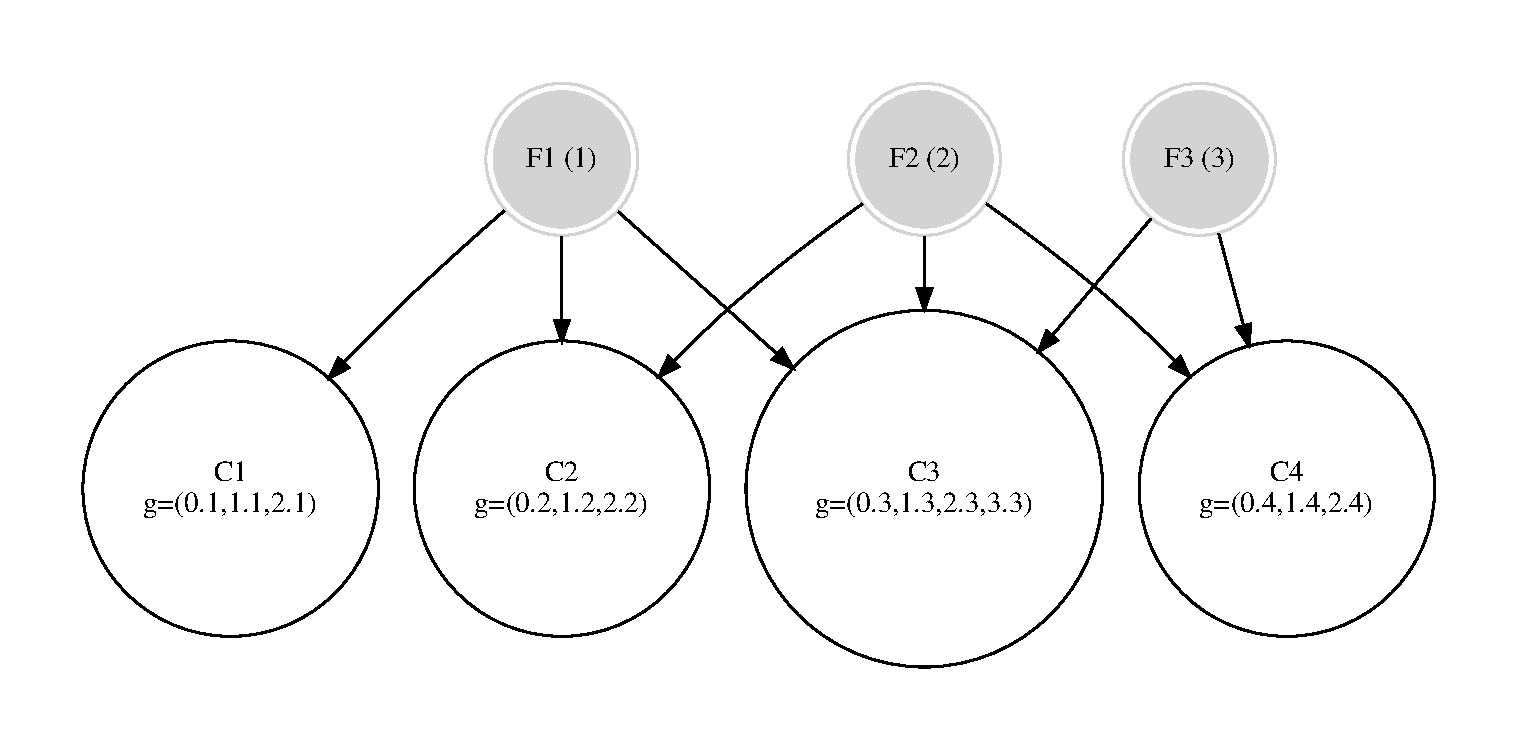
\includegraphics[width=0.8\textwidth]{./problem_dia.gv.pdf}
\caption{Problem description: facilty location with overlaps. \\
\textbf{Facilities:} numbers in parentheses indicate switch-on costs.\\
\textbf{Consumers:} overlap penalies are shown, $g=(0,1,2)$ would mean that for this consumer zero
overlapping coverings imposed no additional cost, covering with one facility brought additional cost $1$,
with two facilities (i.e., actual overlap) brought cost $2$. These numbers are chosen to be the same for
all consumers (no restrictions to change this, just for simplicity).}
\label{fig:problem}
\end{figure}

I am representing this (or any other) problem in the following three ways.
\subsection{Simple MIP}
\label{sec:org36e1646}
I generate a "naive" MIP right away:
\begin{flalign*}
    \textrm{Minimize:} & 1.0 + x_{1} + 2.0 x_{2} + 3.0 x_{3} + v^1_1 + v^1_2 + 1.0 v^2_2 + v^1_3 + 1.0 v^2_3 + v^3_3 + 1.0 v^1_4 + v^2_4\\
    \textrm{Subject To:} &\\
& -1.0 x_{1} + z_{1\rightarrow 1} = 0.0\\
& -1.0 x_{1} + z_{1\rightarrow 2} = 0.0\\
& -1.0 x_{1} + z_{1\rightarrow 3} = 0.0\\
& -1.0 x_{2} + z_{2\rightarrow 2} = 0.0\\
& -1.0 x_{2} + z_{2\rightarrow 3} = 0.0\\
& -1.0 x_{2} + z_{2\rightarrow 4} = 0.0\\
& -1.0 x_{3} + z_{3\rightarrow 3} = 0.0\\
& -1.0 x_{3} + z_{3\rightarrow 4} = 0.0\\
& -1.0 z_{1\rightarrow 1} + b_{1} = 0.0\\
& -1.0 z_{1\rightarrow 2} -1.0 z_{2\rightarrow 2} + b_{2} = 0.0\\
& -1.0 z_{1\rightarrow 3} -1.0 z_{2\rightarrow 3} -1.0 z_{3\rightarrow 3} + b_{3} = 0.0\\
& -1.0 z_{2\rightarrow 4} -1.0 z_{3\rightarrow 4} + b_{4} = 0.0\\
& b_{1} -1.0 v^1_1 = 0.0\\
& -1.0 v^1_2 + v^2_2 \leq 0.0\\
& b_{2} -1.0 v^1_2 -1.0 v^2_2 = 0.0\\
& -1.0 v^1_3 + v^2_3 \leq 0.0\\
& -1.0 v^2_3 + v^3_3 \leq 0.0\\
& b_{3} -1.0 v^1_3 -1.0 v^2_3 -1.0 v^3_3 = 0.0\\
& -1.0 v^1_4 + v^2_4 \leq 0.0\\
& b_{4} -1.0 v^1_4 -1.0 v^2_4 = 0.0,
\end{flalign*}
where \(x\) are "locate" decisions, \(z\) are covering decisions (which are kind of
dependent on each other, like we discussed), \(b\) are numbers of overlaps, and
\(v\) are used to encode an arbitrary overlap penalty function.

Binary variables are:
\([x_{1}, z_{1\rightarrow 1}, z_{1\rightarrow 2},
z_{1\rightarrow 3}, x_{2}, z_{2\rightarrow 2}, z_{2\rightarrow 3},
z_{2\rightarrow 4}, x_{3}, z_{3\rightarrow 3}, z_{3\rightarrow 4}, v^1_1, v^1_2,
v^2_2, v^1_3, v^2_3, v^3_3, v^1_4, v^2_4]\) (and I kind of hope that Gurobi's
\texttt{presolve} takes care of the redundant variables.)

\subsection{CPP MIP}
\label{sec:orgf3ee3b1}
Now, I am generating two decision diagrams, as before:

\begin{center}
\begin{tabular}{llll}
\textbf{Diagram} & \textbf{Constraints incorporated} & \textbf{Costs incorporated} & \textbf{Figure}\\
\hline
\hline
Covering & Cover each consumer & \(c_{ij}\) (covering) & \ref{fig:cover}\\
 & at least once & \(g_j(n_j)\) (overlap) & \\
\hline
Availability & "Switch-on" and "covering" & \(f_i\) (switch-on) & \ref{fig:avail}\\
 & variables are consistent &  & \\
\hline
\end{tabular}
\end{center}

\begin{figure}[t!]
  \begin{subfigure}[t]{0.45\textwidth}
    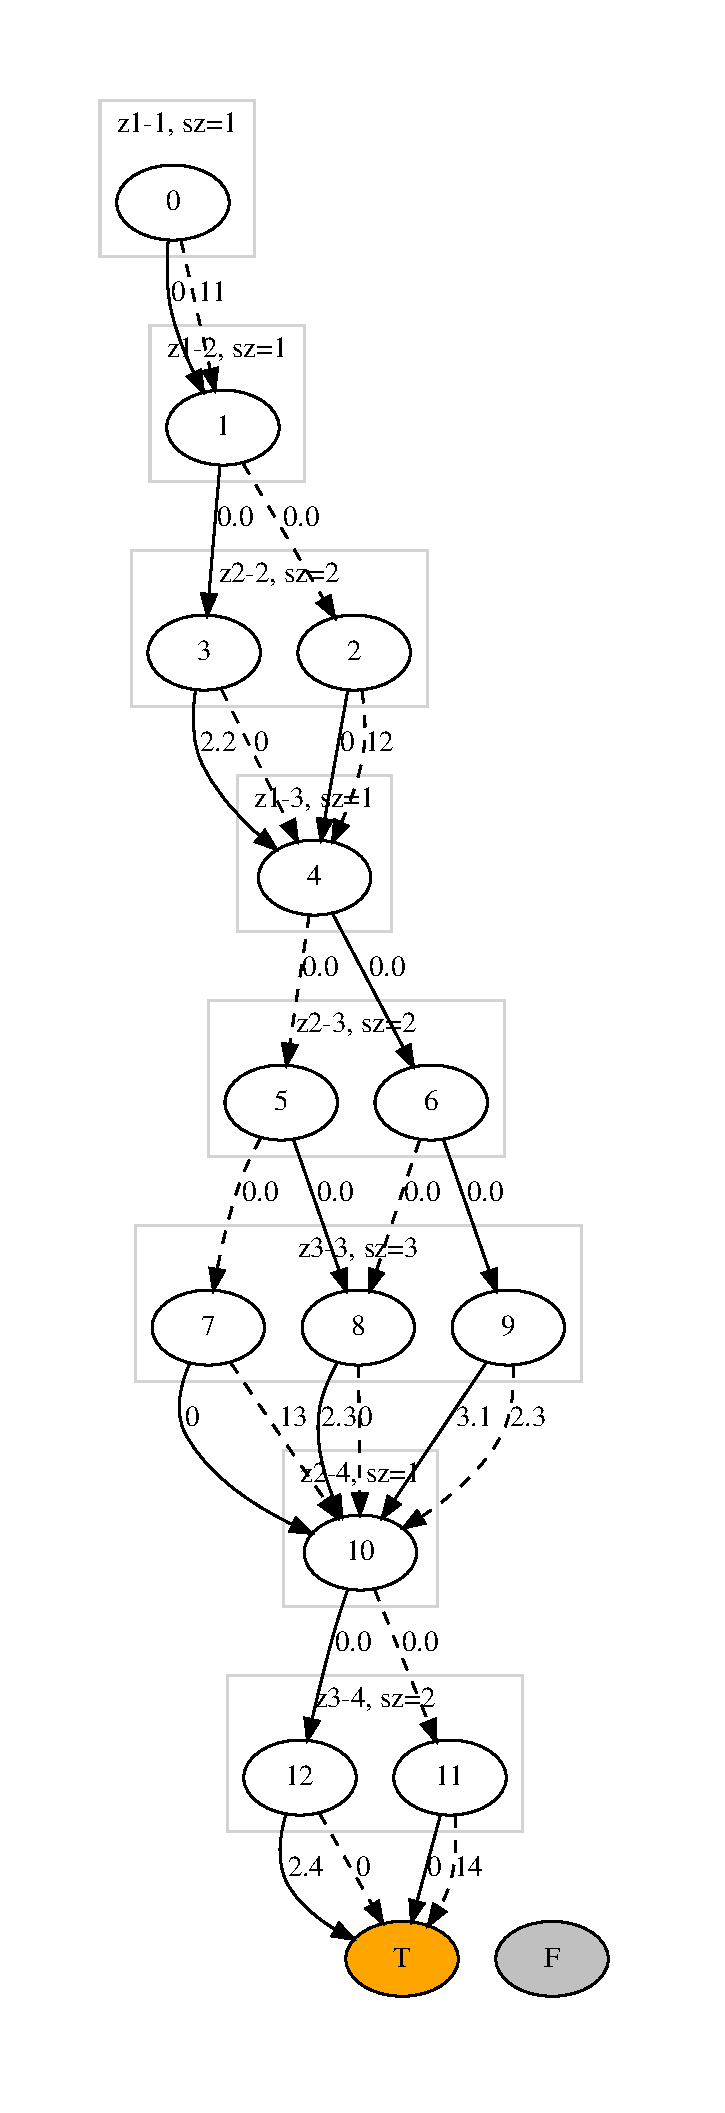
\includegraphics[height=\textheight]{./covering.dot.pdf}
    \caption{Covering BDD}\label{fig:cover}
  \end{subfigure}%
  \hfill
  \begin{subfigure}[t]{0.45\textwidth}
    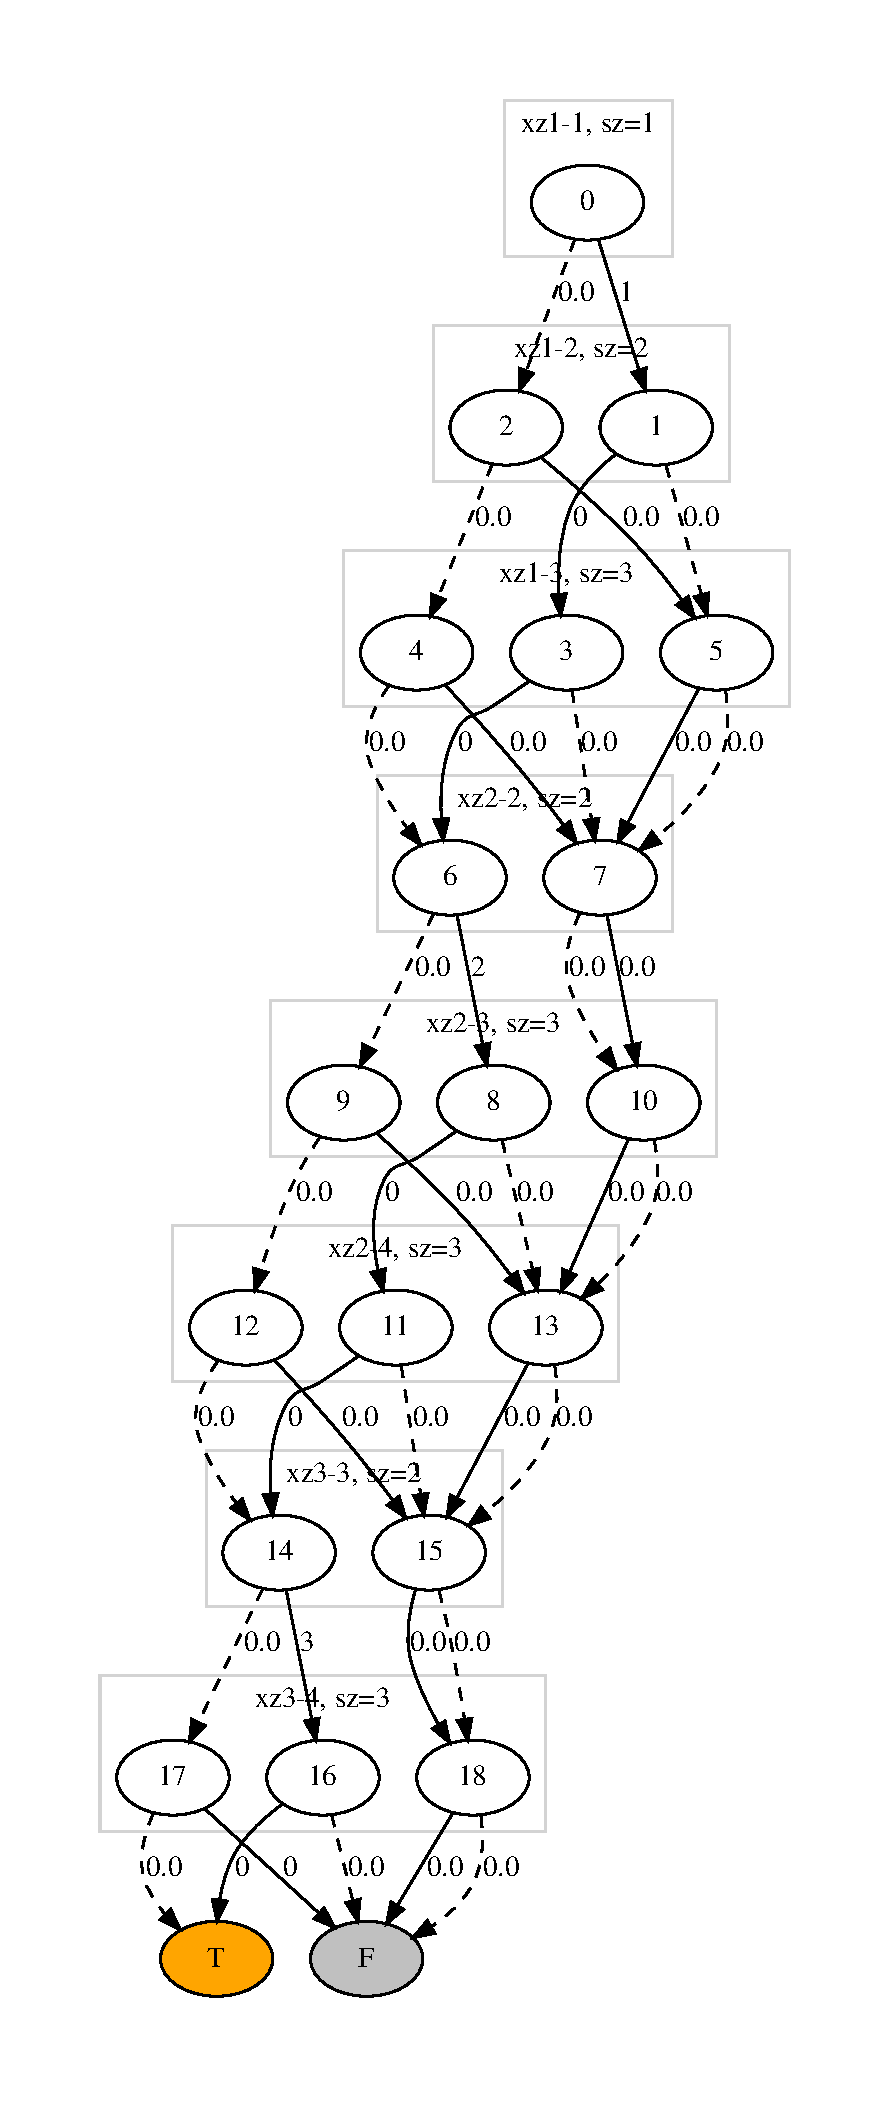
\includegraphics[height=\textheight]{./availability.dot.pdf}
    \caption{Availability BDD}\label{fig:avail}
  \end{subfigure}
  \caption{BDDs generated to encode the instance from Figure \ref{fig:problem}.}
\end{figure}

Which allows me to formulate the following MIP:
The objective is:
\begin{flalign*}
\textrm{Minimize:}\quad\quad & v^A_{0\rightarrow 1,h} + 2.0 v^A_{6 \rightarrow 8, h} + 3.0 v^A_{14 \rightarrow 16, h} +\\
& 1.1 v^C_{0 \rightarrow 1, h} + 0.1 v^C_{0 \rightarrow 1, l} + 1.2 v^C_{2 \rightarrow 4, h} + 0.2 v^C_{2 \rightarrow 4, l} + 2.2 v^C_{3 \rightarrow 4, h} + 1.2 v^C_{3 \rightarrow 4, l} + \\
& 1.3 v^C_{7 \rightarrow 10, h} + 0.3 v^C_{7 \rightarrow 10, l} + 3.3 v^C_{9 \rightarrow 10, h} + 2.3 v^C_{9 \rightarrow 10, l} + 2.3 v^C_{8 \rightarrow 10, h} + 1.3 v^C_{8 \rightarrow 10, l} + \\
& 2.4 v^C_{12 \rightarrow T, h} + 1.4 v^C_{12 \rightarrow T, l} + 1.4 v^C_{11 \rightarrow T, h} + 0.4 v^C_{11 \rightarrow T, l}.
\end{flalign*}

Here, for example, variable \(v^A_{0\rightarrow 1,h}\) corresponds to the flow
from node \textcircled{0} to node \textcircled{1} of diagram \(A\) (availability),
along the "hi" ("yes") arc.\\

\textbf{Legend.}
\begin{itemize}
\item From each diagram, two types of constraints are generated:
\begin{itemize}
\item \emph{cont-at-\textcircled{.}} are flow continuity constraints at a given node.
\item \emph{bin-link-<k>} are binary linking constraints (needed to link two BDDs -- i.e.,
tangle network flow problems), one per layer, indexed with \(k\).
\end{itemize}
\item \(A\) denotes "Availability" diagram, \(C\) denotes "Covering"
diagram.
\end{itemize}

All node numbers correspond to the diagrams and have nothing to do with
customer and facility indices.

\begin{itemize}
\item Arc flow variables (continuous) \(v\).
\item Linking variables (binary): \(\lambda_{z1-1}, \lambda_{z1-2}, \lambda_{z1-3}, \lambda_{z2-2}, \lambda_{z2-3}, \lambda_{z2-4}, \lambda_{z3-3}, \lambda_{z3-4}\).
\end{itemize}

\newpage Constraints from \textbf{covering BDD}:\\

\begin{tabular}{l l}
\textbf{Type} & \textbf{Constraint}\\\hline\\
    cont-at-0 & $-1.0 v^A_{0 \rightarrow 1, h} -1.0 v^A_{0 \rightarrow 2, l} = -1.0$\\
    bin-link-1 & $\lambda_{z1-1} -1.0 v^A_{0 \rightarrow 1, h} = 0.0$\\
    cont-at-2 & $v^A_{0 \rightarrow 2, l} -1.0 v^A_{2 \rightarrow 5, h} -1.0 v^A_{2 \rightarrow 4, l} = 0.0$\\
    cont-at-1 & $v^A_{0 \rightarrow 1, h} -1.0 v^A_{1 \rightarrow 3, h} -1.0 v^A_{1 \rightarrow 5, l} = 0.0$\\
    bin-link-2 & $\lambda_{z1-2} -1.0 v^A_{2 \rightarrow 5, h} -1.0 v^A_{1 \rightarrow 3, h} = 0.0$\\
    cont-at-3 & $v^A_{1 \rightarrow 3, h} -1.0 v^A_{3 \rightarrow 6, h} -1.0 v^A_{3 \rightarrow 7, l} = 0.0$\\
    cont-at-4 & $v^A_{2 \rightarrow 4, l} -1.0 v^A_{4 \rightarrow 7, h} -1.0 v^A_{4 \rightarrow 6, l} = 0.0$\\
    cont-at-5 & $v^A_{2 \rightarrow 5, h} + v^A_{1 \rightarrow 5, l} -1.0 v^A_{5 \rightarrow 7, h} -1.0 v^A_{5 \rightarrow 7, l} = 0.0$\\
    bin-link-3 & $\lambda_{z1-3} -1.0 v^A_{3 \rightarrow 6, h} -1.0 v^A_{4 \rightarrow 7, h} -1.0 v^A_{5 \rightarrow 7, h} = 0.0$\\
    cont-at-7 & $v^A_{3 \rightarrow 7, l} + v^A_{4 \rightarrow 7, h} + v^A_{5 \rightarrow 7, h} + v^A_{5 \rightarrow 7, l} -1.0 v^A_{7 \rightarrow 10, h} -1.0 v^A_{7 \rightarrow 10, l} = 0.0$\\
    cont-at-6 & $v^A_{3 \rightarrow 6, h} + v^A_{4 \rightarrow 6, l} -1.0 v^A_{6 \rightarrow 8, h} -1.0 v^A_{6 \rightarrow 9, l} = 0.0$\\
    bin-link-4 & $\lambda_{z2-2} -1.0 v^A_{7 \rightarrow 10, h} -1.0 v^A_{6 \rightarrow 8, h} = 0.0$\\
    cont-at-10 & $v^A_{7 \rightarrow 10, h} + v^A_{7 \rightarrow 10, l} -1.0 v^A_{10 \rightarrow 13, h} -1.0 v^A_{10 \rightarrow 13, l} = 0.0$\\
    cont-at-9 & $v^A_{6 \rightarrow 9, l} -1.0 v^A_{9 \rightarrow 13, h} -1.0 v^A_{9 \rightarrow 12, l} = 0.0$\\
    cont-at-8 & $v^A_{6 \rightarrow 8, h} -1.0 v^A_{8 \rightarrow 11, h} -1.0 v^A_{8 \rightarrow 13, l} = 0.0$\\
    bin-link-5 & $\lambda_{z2-3} -1.0 v^A_{10 \rightarrow 13, h} -1.0 v^A_{9 \rightarrow 13, h} -1.0 v^A_{8 \rightarrow 11, h} = 0.0$\\
    cont-at-12 & $v^A_{9 \rightarrow 12, l} -1.0 v^A_{12 \rightarrow 15, h} -1.0 v^A_{12 \rightarrow 14, l} = 0.0$\\
    cont-at-13 & $v^A_{10 \rightarrow 13, h} + v^A_{10 \rightarrow 13, l} + v^A_{9 \rightarrow 13, h} + v^A_{8 \rightarrow 13, l} -1.0 v^A_{13 \rightarrow 15, h} -1.0 v^A_{13 \rightarrow 15, l} = 0.0$\\
    cont-at-11 & $v^A_{8 \rightarrow 11, h} -1.0 v^A_{11 \rightarrow 14, h} -1.0 v^A_{11 \rightarrow 15, l} = 0.0$\\
    bin-link-6 & $\lambda_{z2-4} -1.0 v^A_{12 \rightarrow 15, h} -1.0 v^A_{13 \rightarrow 15, h} -1.0 v^A_{11 \rightarrow 14, h} = 0.0$\\
    cont-at-14 & $v^A_{12 \rightarrow 14, l} + v^A_{11 \rightarrow 14, h} -1.0 v^A_{14 \rightarrow 16, h} -1.0 v^A_{14 \rightarrow 17, l} = 0.0$\\
    cont-at-15 & $v^A_{12 \rightarrow 15, h} + v^A_{13 \rightarrow 15, h} + v^A_{13 \rightarrow 15, l} + v^A_{11 \rightarrow 15, l} -1.0 v^A_{15 \rightarrow 18, h} -1.0 v^A_{15 \rightarrow 18, l} = 0.0$\\
    bin-link-7 & $\lambda_{z3-3} -1.0 v^A_{14 \rightarrow 16, h} -1.0 v^A_{15 \rightarrow 18, h} = 0.0$\\
    cont-at-18 & $v^A_{15 \rightarrow 18, h} + v^A_{15 \rightarrow 18, l} -1.0 v^A_{18 \rightarrow F, h} -1.0 v^A_{18 \rightarrow F, l} = 0.0$\\
    cont-at-17 & $v^A_{14 \rightarrow 17, l} -1.0 v^A_{17 \rightarrow F, h} -1.0 v^A_{17 \rightarrow T, l} = 0.0$\\
    cont-at-16 & $v^A_{14 \rightarrow 16, h} -1.0 v^A_{16 \rightarrow T, h} -1.0 v^A_{16 \rightarrow F, l} = 0.0$\\
    bin-link-8 & $\lambda_{z3-4} -1.0 v^A_{18 \rightarrow F, h} -1.0 v^A_{17 \rightarrow F, h} -1.0 v^A_{16 \rightarrow T, h} = 0.0$\\
    cont-at-T & $v^A_{17 \rightarrow T, l} + v^A_{16 \rightarrow T, h} = 1.0$\\
    cont-at-F & $v^A_{18 \rightarrow F, h} + v^A_{18 \rightarrow F, l} + v^A_{17 \rightarrow F, h} + v^A_{16 \rightarrow F, l} = 0.0$
\end{tabular}

\newpage Constraints from \textbf{availability BBD}\\

\begin{tabular}{l l}
\textbf{Type} & \textbf{Constraint}\\\hline\\
    cont-at-0 & $-1.0 v^C_{0 \rightarrow 1, h} -1.0 v^C_{0 \rightarrow 1, l} = -1.0$\\
    bin-link-1 & $\lambda_{z1-1} -1.0 v^C_{0 \rightarrow 1, h} = 0.0$\\
    cont-at-1 & $v^C_{0 \rightarrow 1, h} + v^C_{0 \rightarrow 1, l} -1.0 v^C_{1 \rightarrow 3, h} -1.0 v^C_{1 \rightarrow 2, l} = 0.0$\\
    bin-link-2 & $\lambda_{z1-2} -1.0 v^C_{1 \rightarrow 3, h} = 0.0$\\
    cont-at-2 & $v^C_{1 \rightarrow 2, l} -1.0 v^C_{2 \rightarrow 4, h} -1.0 v^C_{2 \rightarrow 4, l} = 0.0$\\
    cont-at-3 & $v^C_{1 \rightarrow 3, h} -1.0 v^C_{3 \rightarrow 4, h} -1.0 v^C_{3 \rightarrow 4, l} = 0.0$\\
    bin-link-3 & $\lambda_{z2-2} -1.0 v^C_{2 \rightarrow 4, h} -1.0 v^C_{3 \rightarrow 4, h} = 0.0$\\
    cont-at-4 & $v^C_{2 \rightarrow 4, h} + v^C_{2 \rightarrow 4, l} + v^C_{3 \rightarrow 4, h} + v^C_{3 \rightarrow 4, l} -1.0 v^C_{4 \rightarrow 6, h} -1.0 v^C_{4 \rightarrow 5, l} = 0.0$\\
    bin-link-4 & $\lambda_{z1-3} -1.0 v^C_{4 \rightarrow 6, h} = 0.0$\\
    cont-at-5 & $v^C_{4 \rightarrow 5, l} -1.0 v^C_{5 \rightarrow 8, h} -1.0 v^C_{5 \rightarrow 7, l} = 0.0$\\
    cont-at-6 & $v^C_{4 \rightarrow 6, h} -1.0 v^C_{6 \rightarrow 9, h} -1.0 v^C_{6 \rightarrow 8, l} = 0.0$\\
    bin-link-5 & $\lambda_{z2-3} -1.0 v^C_{5 \rightarrow 8, h} -1.0 v^C_{6 \rightarrow 9, h} = 0.0$\\
    cont-at-7 & $v^C_{5 \rightarrow 7, l} -1.0 v^C_{7 \rightarrow 10, h} -1.0 v^C_{7 \rightarrow 10, l} = 0.0$\\
    cont-at-9 & $v^C_{6 \rightarrow 9, h} -1.0 v^C_{9 \rightarrow 10, h} -1.0 v^C_{9 \rightarrow 10, l} = 0.0$\\
    cont-at-8 & $v^C_{5 \rightarrow 8, h} + v^C_{6 \rightarrow 8, l} -1.0 v^C_{8 \rightarrow 10, h} -1.0 v^C_{8 \rightarrow 10, l} = 0.0$\\
    bin-link-6 & $\lambda_{z3-3} -1.0 v^C_{7 \rightarrow 10, h} -1.0 v^C_{9 \rightarrow 10, h} -1.0 v^C_{8 \rightarrow 10, h} = 0.0$\\
    cont-at-10 & $v^C_{7 \rightarrow 10, h} + v^C_{7 \rightarrow 10, l} + v^C_{9 \rightarrow 10, h} + v^C_{9 \rightarrow 10, l} + v^C_{8 \rightarrow 10, h} + v^C_{8 \rightarrow 10, l} -1.0 v^C_{10 \rightarrow 12, h} -1.0 v^C_{10 \rightarrow 11, l} = 0.0$\\
    bin-link-7 & $\lambda_{z2-4} -1.0 v^C_{10 \rightarrow 12, h} = 0.0$\\
    cont-at-12 & $v^C_{10 \rightarrow 12, h} -1.0 v^C_{12 \rightarrow T, h} -1.0 v^C_{12 \rightarrow T, l} = 0.0$\\
    cont-at-11 & $v^C_{10 \rightarrow 11, l} -1.0 v^C_{11 \rightarrow T, h} -1.0 v^C_{11 \rightarrow T, l} = 0.0$\\
    bin-link-8 & $\lambda_{z3-4} -1.0 v^C_{12 \rightarrow T, h} -1.0 v^C_{11 \rightarrow T, h} = 0.0$\\
    cont-at-F & $0.0 = 0.0$\\
    cont-at-T & $v^C_{12 \rightarrow T, h} + v^C_{12 \rightarrow T, l} + v^C_{11 \rightarrow T, h} + v^C_{11 \rightarrow T, l} = 1.0$\\
\end{tabular}

\subsection{Intersection BDD}
\label{sec:org3092701}
This is a little more tricky. First, I make 'availability' and 'covering' diagrams order-associated:

\begin{minted}[frame=lines,fontsize=\scriptsize,xleftmargin=\parindent,linenos]{python}
import varseq as vs
from BB_search import BBSearch

print(f"Size *before* alignment: {A.size()} + {C.size()} = {A.size() + C.size()} nodes.")
vs_A = vs.VarSeq(A.vars, [len(L) for L in A.layers[:-1]])
vs_C = vs.VarSeq(C.vars, [len(L) for L in C.layers[:-1]])
b = BBSearch(vs_A, vs_C)

status = b.search()
assert status == "optimal" or status == "timeout"

Ap = A.align_to(b.Ap_cand.layer_var, inplace=False)
Cp = C.align_to(b.Ap_cand.layer_var, inplace=False)

Ap.show(dir="reports/2021-02-23_Status_BM/", filename="A_aligned.dot")
Cp.show(dir="reports/2021-02-23_Status_BM/", filename="C_aligned.dot")
print(f"Size *after* alignment: {Ap.size()} + {Cp.size()} = {Ap.size() + Cp.size()} nodes.")
print(f"The order revised from \n A: {A.vars}, and\n C: {C.vars}...")
print(f"...to {Ap.vars}")
\end{minted}

\begin{verbatim}
Size *before* alignment: 19 + 13 = 32 nodes.
Size *after* alignment: 22 + 14 = 36 nodes.
The order revised from 
 A: ['z1-1', 'z1-2', 'z1-3', 'z2-2', 'z2-3', 'z2-4', 'z3-3', 'z3-4'], and
 C: ['z1-1', 'z1-2', 'z2-2', 'z1-3', 'z2-3', 'z3-3', 'z2-4', 'z3-4']...
...to ['z1-1', 'z1-2', 'z1-3', 'z2-2', 'z2-3', 'z3-3', 'z2-4', 'z3-4']
\end{verbatim}


(This results in the diagrams depicted in Figures \ref{fig:coverA} and \ref{fig:availA}, respectively.)

\begin{figure}[t!]
  \begin{subfigure}[t]{0.45\textwidth}
    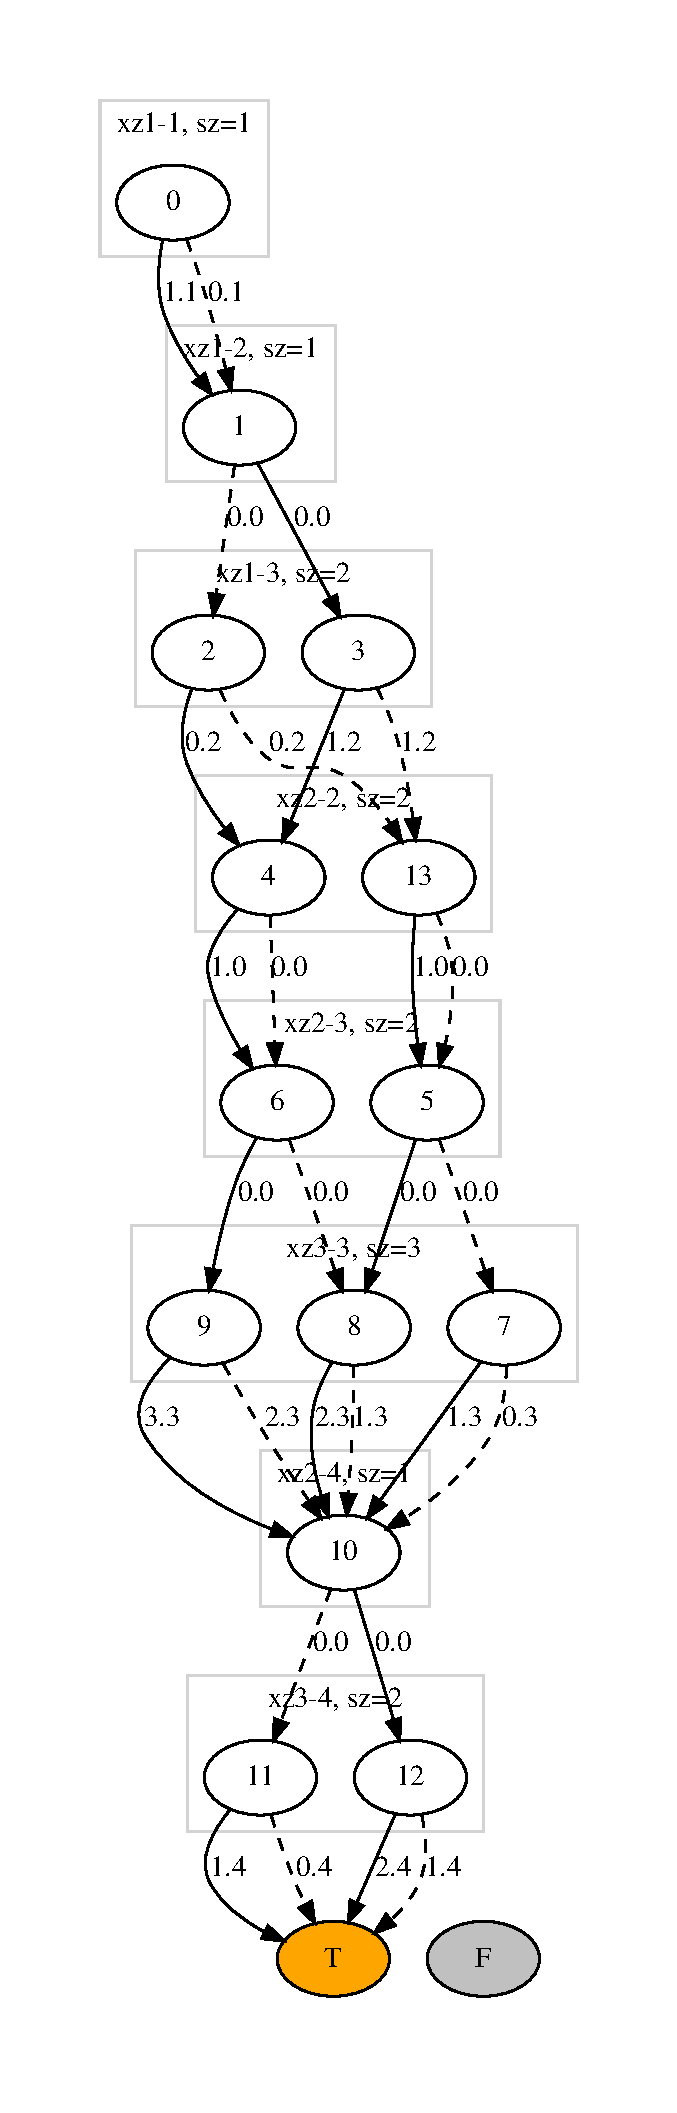
\includegraphics[height=\textheight]{./C_aligned.dot.pdf}
    \caption{Covering BDD}\label{fig:coverA}
  \end{subfigure}%
  \hfill
  \begin{subfigure}[t]{0.45\textwidth}
    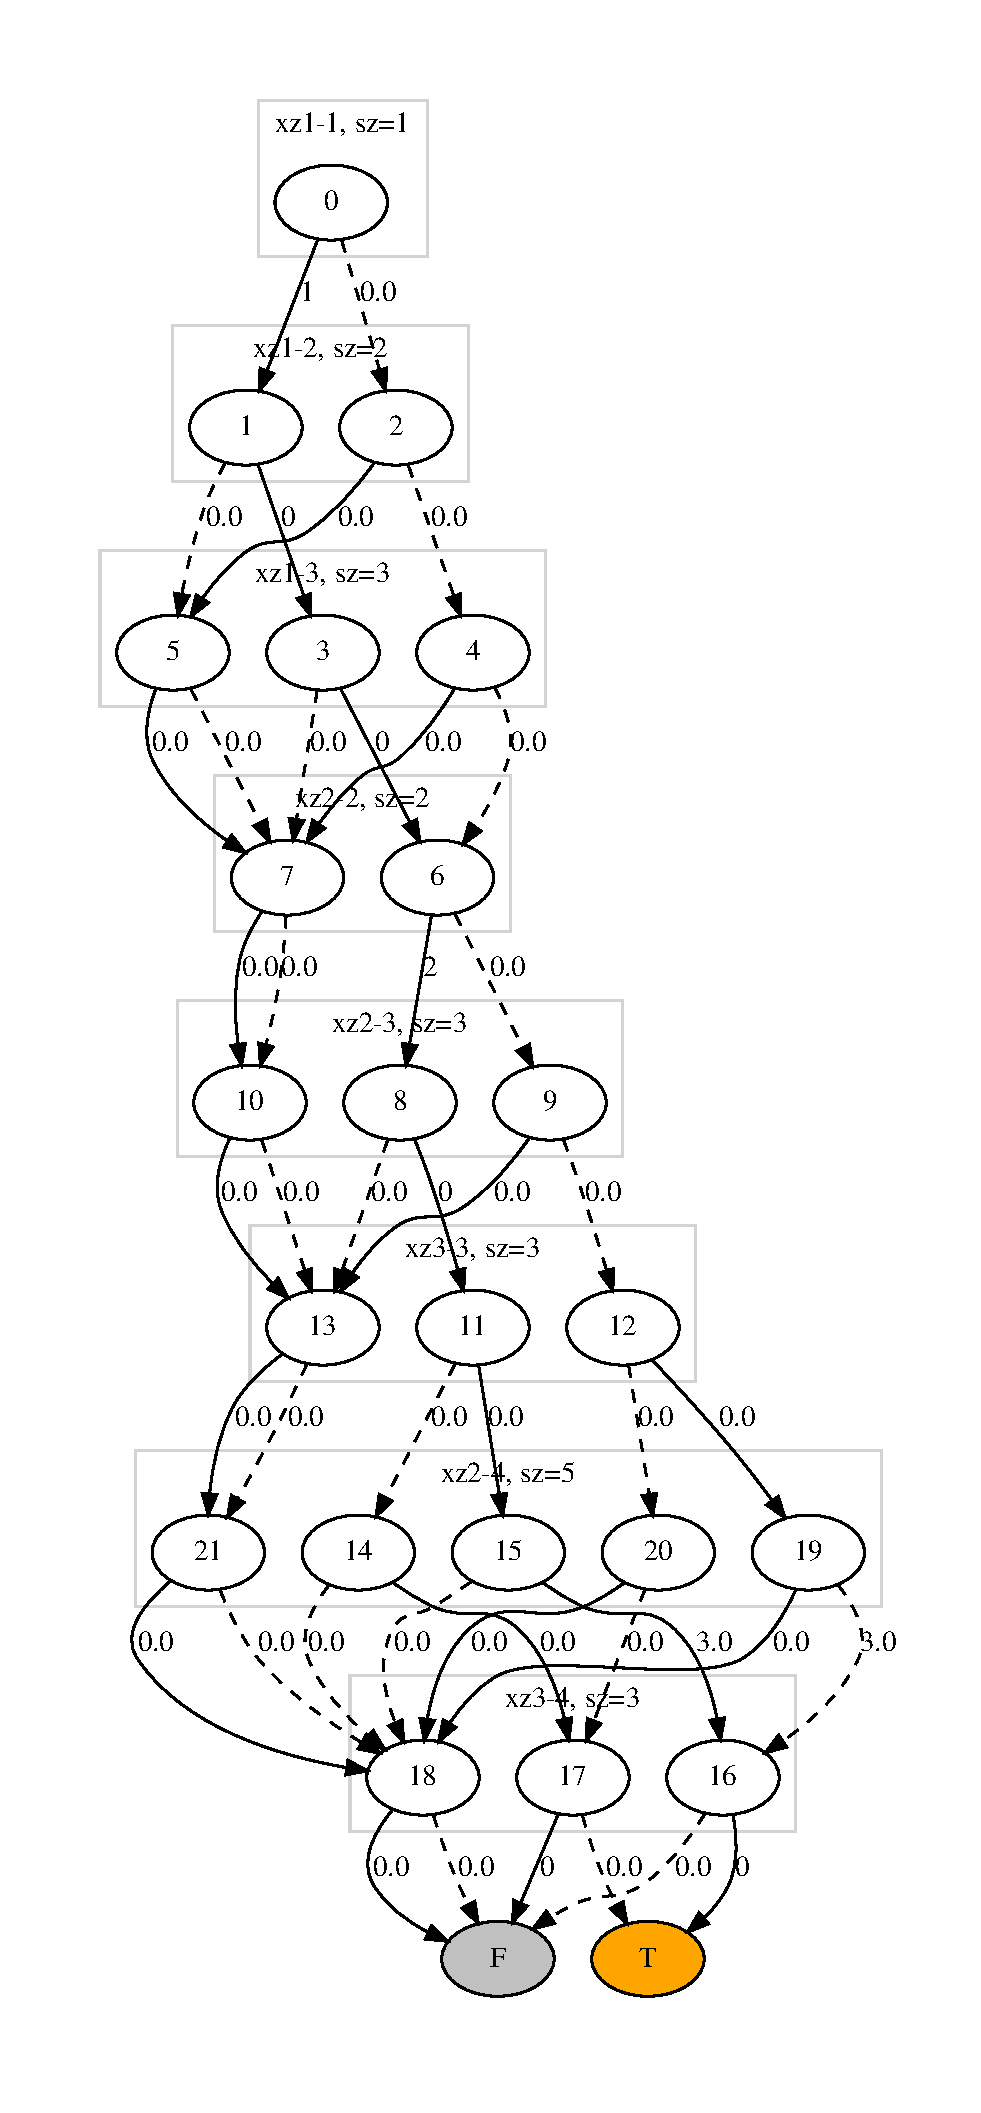
\includegraphics[height=\textheight]{./A_aligned.dot.pdf}
    \caption{Availability BDD}\label{fig:availA}
  \end{subfigure}
  \caption{BDDs generated to encode the instance from Figure \ref{fig:problem}: after alignment.}
\end{figure}

So, I can generate an intersection BDD (Figure \ref{fig:intDD}) and the corresponding MIP:

\begin{figure}[h!]
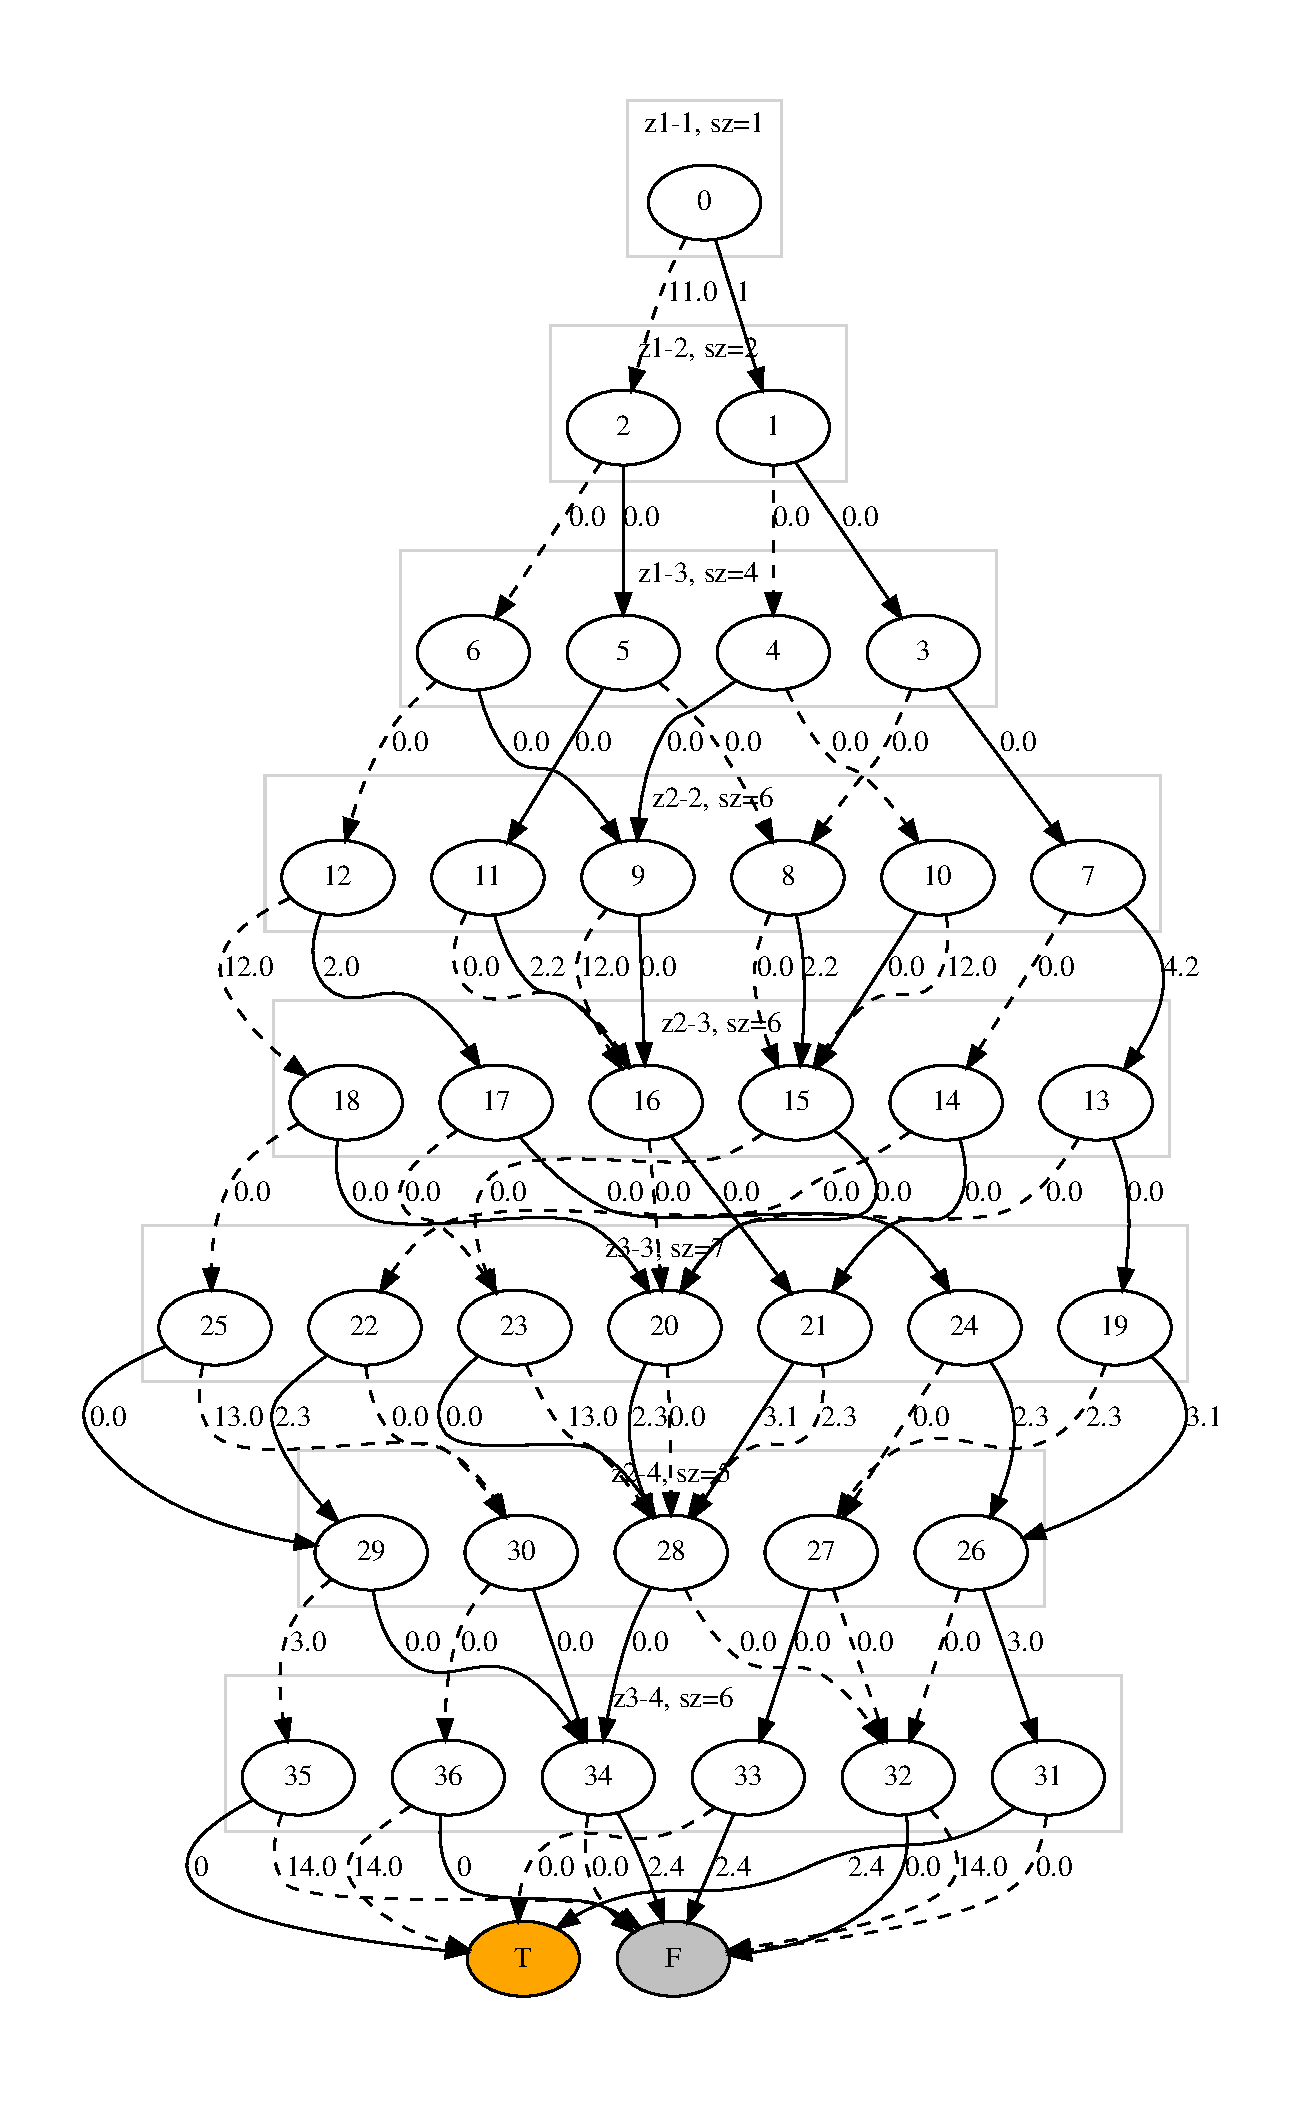
\includegraphics[width=0.9\textwidth]{./intersection.dot.pdf}
\caption{An intersection diagram for 'availability' and 'covering' DDs.}
\label{fig:intDD}
\end{figure}

The objective is:
\begin{flalign*}
\textrm{Minimize: } & 2.1 v_{0 \rightarrow 1, h} + 0.1 v_{0 \rightarrow 2, l} + 0.2 v_{6 \rightarrow 9, h} + 0.2 v_{6 \rightarrow 10, l} + 1.2 v_{5 \rightarrow 9, h} + \\
& 1.2 v_{5 \rightarrow 8, l} + 0.2 v_{4 \rightarrow 9, h} + 0.2 v_{4 \rightarrow 8, l} + 1.2 v_{3 \rightarrow 7, h} + 1.2 v_{3 \rightarrow 8, l} + 3.0 v_{10 \rightarrow 15, h} +\\
& 3.0 v_{7 \rightarrow 11, h} + v_{9 \rightarrow 14, h} + v_{8 \rightarrow 13, h} + 1.3 v_{21 \rightarrow 26, h} + 0.3 v_{21 \rightarrow 26, l} + 3.3 v_{17 \rightarrow 24, h} + \\
& 2.3 v_{17 \rightarrow 25, l} + 2.3 v_{22 \rightarrow 24, h} + 1.3 v_{22 \rightarrow 25, l} + 3.3 v_{19 \rightarrow 26, h} + 2.3 v_{19 \rightarrow 26, l} +\\
& 1.3 v_{23 \rightarrow 27, h} + 0.3 v_{23 \rightarrow 28, l} + 2.3 v_{18 \rightarrow 26, h} + 1.3 v_{18 \rightarrow 26, l} + 2.3 v_{20 \rightarrow 27, h} +\\
& 1.3 v_{20 \rightarrow 28, l} + 3.0 v_{27 \rightarrow 33, l} + 3.0 v_{24 \rightarrow 29, h} + 1.4 v_{34 \rightarrow F, h} + 0.4 v_{34 \rightarrow T, l} + \\
& 1.4 v_{30 \rightarrow F, h} + 0.4 v_{30 \rightarrow F, l} + 2.4 v_{29 \rightarrow T, h} + 1.4 v_{29 \rightarrow F, l} + 1.4 v_{33 \rightarrow T, h} + 0.4 v_{33 \rightarrow F, l} +\\
& 2.4 v_{32 \rightarrow F, h} + 1.4 v_{32 \rightarrow F, l} + 2.4 v_{31 \rightarrow F, h} + 1.4 v_{31 \rightarrow T, l},
\end{flalign*}

under the constraints, presented in Table \ref{tab:NFconstr}. Obviously, here I
have continuous variables only.

\begin{table}[ht]
\caption{Network flow constraints (for the intersection BDD).}
 \begin{tabular}{l l}
 \textbf{Type} & \textbf{Constraint}\\\hline\\
   cont-at-0 & $-1.0 v_{0 \rightarrow 1, h} -1.0 v_{0 \rightarrow 2, l} = -1.0$\\
   cont-at-1 & $v_{0 \rightarrow 1, h} -1.0 v_{1 \rightarrow 3, h} -1.0 v_{1 \rightarrow 4, l} = 0.0$\\
   cont-at-2 & $v_{0 \rightarrow 2, l} -1.0 v_{2 \rightarrow 5, h} -1.0 v_{2 \rightarrow 6, l} = 0.0$\\
   cont-at-6 & $v_{2 \rightarrow 6, l} -1.0 v_{6 \rightarrow 9, h} -1.0 v_{6 \rightarrow 10, l} = 0.0$\\
   cont-at-5 & $v_{2 \rightarrow 5, h} -1.0 v_{5 \rightarrow 9, h} -1.0 v_{5 \rightarrow 8, l} = 0.0$\\
   cont-at-4 & $v_{1 \rightarrow 4, l} -1.0 v_{4 \rightarrow 9, h} -1.0 v_{4 \rightarrow 8, l} = 0.0$\\
   cont-at-3 & $v_{1 \rightarrow 3, h} -1.0 v_{3 \rightarrow 7, h} -1.0 v_{3 \rightarrow 8, l} = 0.0$\\
   cont-at-10 & $v_{6 \rightarrow 10, l} -1.0 v_{10 \rightarrow 15, h} -1.0 v_{10 \rightarrow 16, l} = 0.0$\\
   cont-at-7 & $v_{3 \rightarrow 7, h} -1.0 v_{7 \rightarrow 11, h} -1.0 v_{7 \rightarrow 12, l} = 0.0$\\
   cont-at-9 & $v_{6 \rightarrow 9, h} + v_{5 \rightarrow 9, h} + v_{4 \rightarrow 9, h} -1.0 v_{9 \rightarrow 14, h} -1.0 v_{9 \rightarrow 14, l} = 0.0$\\
   cont-at-8 & $v_{5 \rightarrow 8, l} + v_{4 \rightarrow 8, l} + v_{3 \rightarrow 8, l} -1.0 v_{8 \rightarrow 13, h} -1.0 v_{8 \rightarrow 13, l} = 0.0$\\
   cont-at-16 & $v_{10 \rightarrow 16, l} -1.0 v_{16 \rightarrow 18, h} -1.0 v_{16 \rightarrow 23, l} = 0.0$\\
   cont-at-11 & $v_{7 \rightarrow 11, h} -1.0 v_{11 \rightarrow 17, h} -1.0 v_{11 \rightarrow 18, l} = 0.0$\\
   cont-at-12 & $v_{7 \rightarrow 12, l} -1.0 v_{12 \rightarrow 19, h} -1.0 v_{12 \rightarrow 20, l} = 0.0$\\
   cont-at-14 & $v_{9 \rightarrow 14, h} + v_{9 \rightarrow 14, l} -1.0 v_{14 \rightarrow 19, h} -1.0 v_{14 \rightarrow 18, l} = 0.0$\\
   cont-at-15 & $v_{10 \rightarrow 15, h} -1.0 v_{15 \rightarrow 22, h} -1.0 v_{15 \rightarrow 21, l} = 0.0$\\
   cont-at-13 & $v_{8 \rightarrow 13, h} + v_{8 \rightarrow 13, l} -1.0 v_{13 \rightarrow 18, h} -1.0 v_{13 \rightarrow 21, l} = 0.0$\\
   cont-at-21 & $v_{15 \rightarrow 21, l} + v_{13 \rightarrow 21, l} -1.0 v_{21 \rightarrow 26, h} -1.0 v_{21 \rightarrow 26, l} = 0.0$\\
   cont-at-17 & $v_{11 \rightarrow 17, h} -1.0 v_{17 \rightarrow 24, h} -1.0 v_{17 \rightarrow 25, l} = 0.0$\\
   cont-at-22 & $v_{15 \rightarrow 22, h} -1.0 v_{22 \rightarrow 24, h} -1.0 v_{22 \rightarrow 25, l} = 0.0$\\
   cont-at-19 & $v_{12 \rightarrow 19, h} + v_{14 \rightarrow 19, h} -1.0 v_{19 \rightarrow 26, h} -1.0 v_{19 \rightarrow 26, l} = 0.0$\\
   cont-at-23 & $v_{16 \rightarrow 23, l} -1.0 v_{23 \rightarrow 27, h} -1.0 v_{23 \rightarrow 28, l} = 0.0$\\
   cont-at-18 & $v_{16 \rightarrow 18, h} + v_{11 \rightarrow 18, l} + v_{14 \rightarrow 18, l} + v_{13 \rightarrow 18, h} -1.0 v_{18 \rightarrow 26, h} -1.0 v_{18 \rightarrow 26, l} = 0.0$\\
   cont-at-20 & $v_{12 \rightarrow 20, l} -1.0 v_{20 \rightarrow 27, h} -1.0 v_{20 \rightarrow 28, l} = 0.0$\\
   cont-at-27 & $v_{23 \rightarrow 27, h} + v_{20 \rightarrow 27, h} -1.0 v_{27 \rightarrow 32, h} -1.0 v_{27 \rightarrow 33, l} = 0.0$\\
   cont-at-25 & $v_{17 \rightarrow 25, l} + v_{22 \rightarrow 25, l} -1.0 v_{25 \rightarrow 31, h} -1.0 v_{25 \rightarrow 30, l} = 0.0$\\
   cont-at-24 & $v_{17 \rightarrow 24, h} + v_{22 \rightarrow 24, h} -1.0 v_{24 \rightarrow 29, h} -1.0 v_{24 \rightarrow 30, l} = 0.0$\\
   cont-at-26 & $v_{21 \rightarrow 26, h} + v_{21 \rightarrow 26, l} + v_{19 \rightarrow 26, h} + v_{19 \rightarrow 26, l} + v_{18 \rightarrow 26, h} + v_{18 \rightarrow 26, l}$\\
   & $-1.0 v_{26 \rightarrow 32, h} -1.0 v_{26 \rightarrow 30, l} = 0.0$\\
   cont-at-28 & $v_{23 \rightarrow 28, l} + v_{20 \rightarrow 28, l} -1.0 v_{28 \rightarrow 32, h} -1.0 v_{28 \rightarrow 34, l} = 0.0$\\
   cont-at-34 & $v_{28 \rightarrow 34, l} -1.0 v_{34 \rightarrow F, h} -1.0 v_{34 \rightarrow T, l} = 0.0$\\
   cont-at-30 & $v_{25 \rightarrow 30, l} + v_{24 \rightarrow 30, l} + v_{26 \rightarrow 30, l} -1.0 v_{30 \rightarrow F, h} -1.0 v_{30 \rightarrow F, l} = 0.0$\\
   cont-at-29 & $v_{24 \rightarrow 29, h} -1.0 v_{29 \rightarrow T, h} -1.0 v_{29 \rightarrow F, l} = 0.0$\\
   cont-at-33 & $v_{27 \rightarrow 33, l} -1.0 v_{33 \rightarrow T, h} -1.0 v_{33 \rightarrow F, l} = 0.0$\\
   cont-at-32 & $v_{27 \rightarrow 32, h} + v_{26 \rightarrow 32, h} + v_{28 \rightarrow 32, h} -1.0 v_{32 \rightarrow F, h} -1.0 v_{32 \rightarrow F, l} = 0.0$\\
   cont-at-31 & $v_{25 \rightarrow 31, h} -1.0 v_{31 \rightarrow F, h} -1.0 v_{31 \rightarrow T, l} = 0.0$\\
   cont-at-T & $v_{34 \rightarrow T, l} + v_{29 \rightarrow T, h} + v_{33 \rightarrow T, h} + v_{31 \rightarrow T, l} = 1.0$\\
   cont-at-F & $v_{34 \rightarrow F, h} + v_{30 \rightarrow F, h} + v_{30 \rightarrow F, l} + v_{29 \rightarrow F, l} + v_{33 \rightarrow F, l} + v_{32 \rightarrow F, h} + v_{32 \rightarrow F, l} + v_{31 \rightarrow F, h} = 0.0$\\
 \end{tabular}
 \label{tab:NFconstr}
\end{table}

\subsection{A quick cross-check}
\label{sec:org337fc6b}
Of course, I'd like to cross-check somehow. E.g., I can just solve each of
the three models and make sure the optimal objective coincide. Indeed:
\begin{verbatim}
Opt statuses are: 2, 2, 2
('optimal' is encoded by 2)
Optimal objectives are:
Simple MIP: 1.0
CPP MIP:    1.0
NF (linear):1.0
\end{verbatim}


Here are, e.g., nonzero variables for the CPP MIP (\texttt{-1} encodes \textbf{True}
terminal node).

\begin{verbatim}
A_vl0_2: 1.0
A_vl2_4: 1.0
A_vl4_6: 1.0
A_vl6_9: 1.0
A_vl9_12: 1.0
A_vl12_14: 1.0
A_vl14_17: 1.0
A_vl17_-1: 1.0
C_vl0_1: 1.0
C_vl1_2: 1.0
C_vl2_4: 1.0
C_vl4_5: 1.0
C_vl5_7: 1.0
C_vl7_10: 1.0
C_vl10_11: 1.0
C_vl11_-1: 1.0
\end{verbatim}

\section{The problem: intersection DD seems to blow up.}
\label{sec:org3d9839a}
What I have done is a very simple experiment: I generated 15 random instances
for different problem sizes -- say, with number of facilities being \(n=3,4,5,6\),
and number of customers \(m=2n\) (in every case). What I have is: diagram sizes
(\(A\) for availability and \(C\) for covering), along with the number of variables
in the plain MIP grow reasonably (Figure \ref{fig:ACsizes}). However,
intersection BDD just blows up (Figure \ref{fig:intSizes} -- note I had to draw it in
\textbf{logarithmic} scale), and so does the runtime of what I am doing (Figure
\ref{fig:runtimes}).

\begin{figure}
  \begin{subfigure}{0.45\textwidth}
    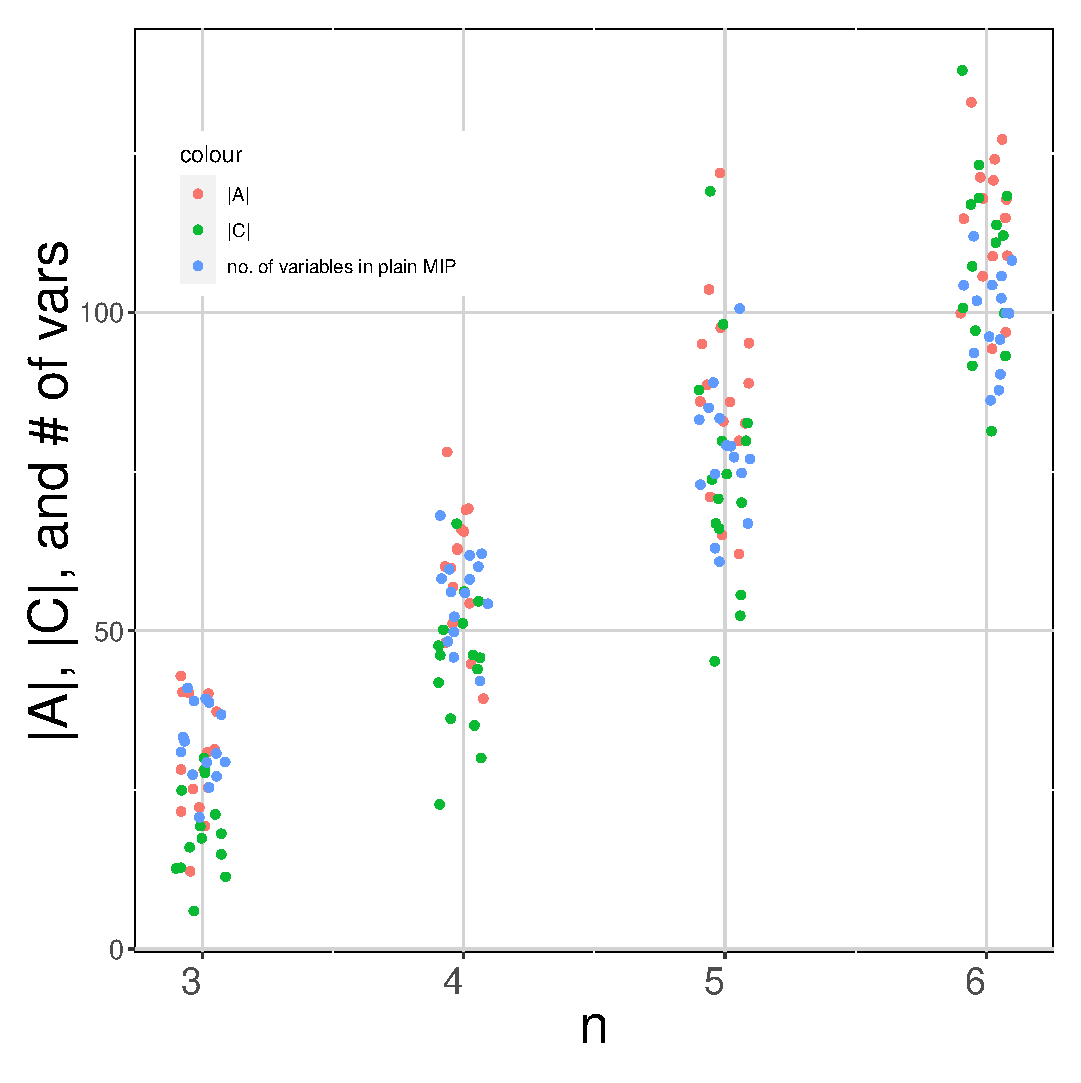
\includegraphics[width=\textwidth]{AandCsizes.eps}
    \caption{Diagram growth as number of facilities increases.}
    \label{fig:ACsizes}
  \end{subfigure}
  \hfill
  \begin{subfigure}{0.45\textwidth}
    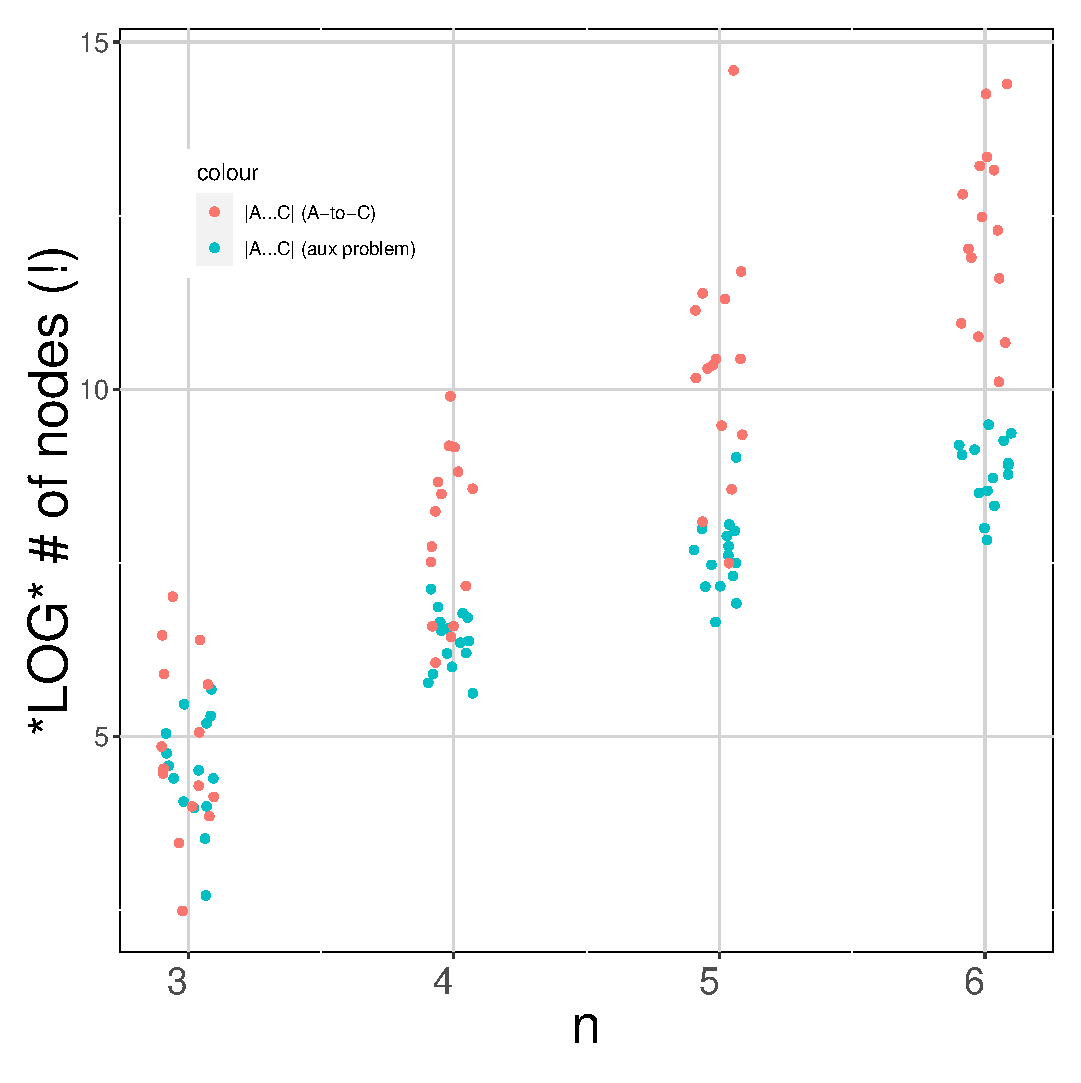
\includegraphics[width=\textwidth]{inter_size.eps}
    \caption{Intersection diagram growth as number of facilities increases.}
    \label{fig:intSizes}
  \end{subfigure}
\end{figure}

\begin{figure}
\center
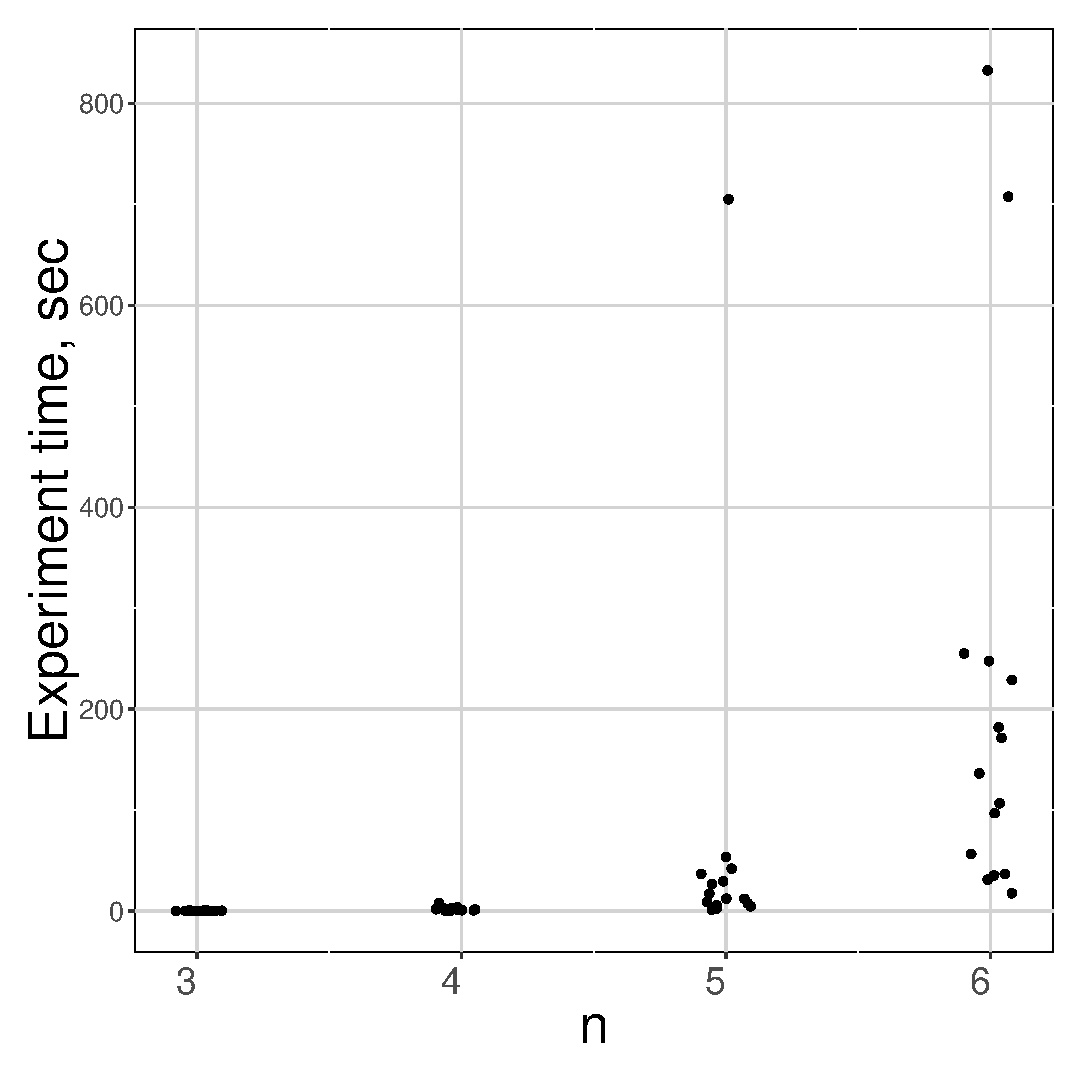
\includegraphics[width=0.7\textwidth]{runtimes.eps}
\caption{Experiment runtimes, seconds}
\label{fig:runtimes}
\end{figure}
\end{document}